\documentclass[a4paper]{article}
\usepackage[utf8]{inputenc}
\usepackage[english]{babel}
\usepackage[T1]{fontenc}
\usepackage{lmodern}
\usepackage{fullpage}
\usepackage{amsmath}
\usepackage{graphicx}
\usepackage{framed}
\usepackage{listings}
\usepackage{placeins}
\usepackage{subcaption}
\usepackage{array}
\usepackage[justification=centering]{caption}

\author{Théotime Grohens}
\title{Introduction to Computer Vision: \\ Assignment 1: Camera Calibration}

\begin{document}

\maketitle

\section*{Question 1}

The projection matrix $M$ that we obtain according to the formulas in the book is:
$$ M =
\begin{pmatrix}
0.004533598809322 & 0.000565451255837 & -0.002028495904507 & 0.523179344403987 \\
0.001842784257069 & -0.004159759032721 & 0.001687792762638 & 0.852192928001303 \\
0.000003256832273 & 0.000001138041825 & 0.000003352377906 & 0.001432092204087
\end{pmatrix}
$$

\section*{Question 2}

The corresponding matrix $K$ of extrinsic parameters is:
$$ K =
\begin{pmatrix}
970.2841013126552  & 0.0986348357588  & 372.0049638053076 \\
                   0   &963.3465813265055  & 299.2920935253743 \\
                   0           &        0 &  1
\end{pmatrix}
$$

\section*{Question 3}

In figure~\ref{11}, we can see the reprojected 3D points drawn alongside with the original 2D input points.
They match quite closely, which empirically means that our estimation of the intrinsic parameters with the linear least-square regression method is pretty good.

The root mean square reproduction error (the root of the average of the squared norms of the difference between input and reprojected points) is then: $e = 0.957354162959341$, which is small compared to the characteristic lengths $u_0$ and $v_0$ of the system (both around 300).

\begin{figure}[h]
\centering
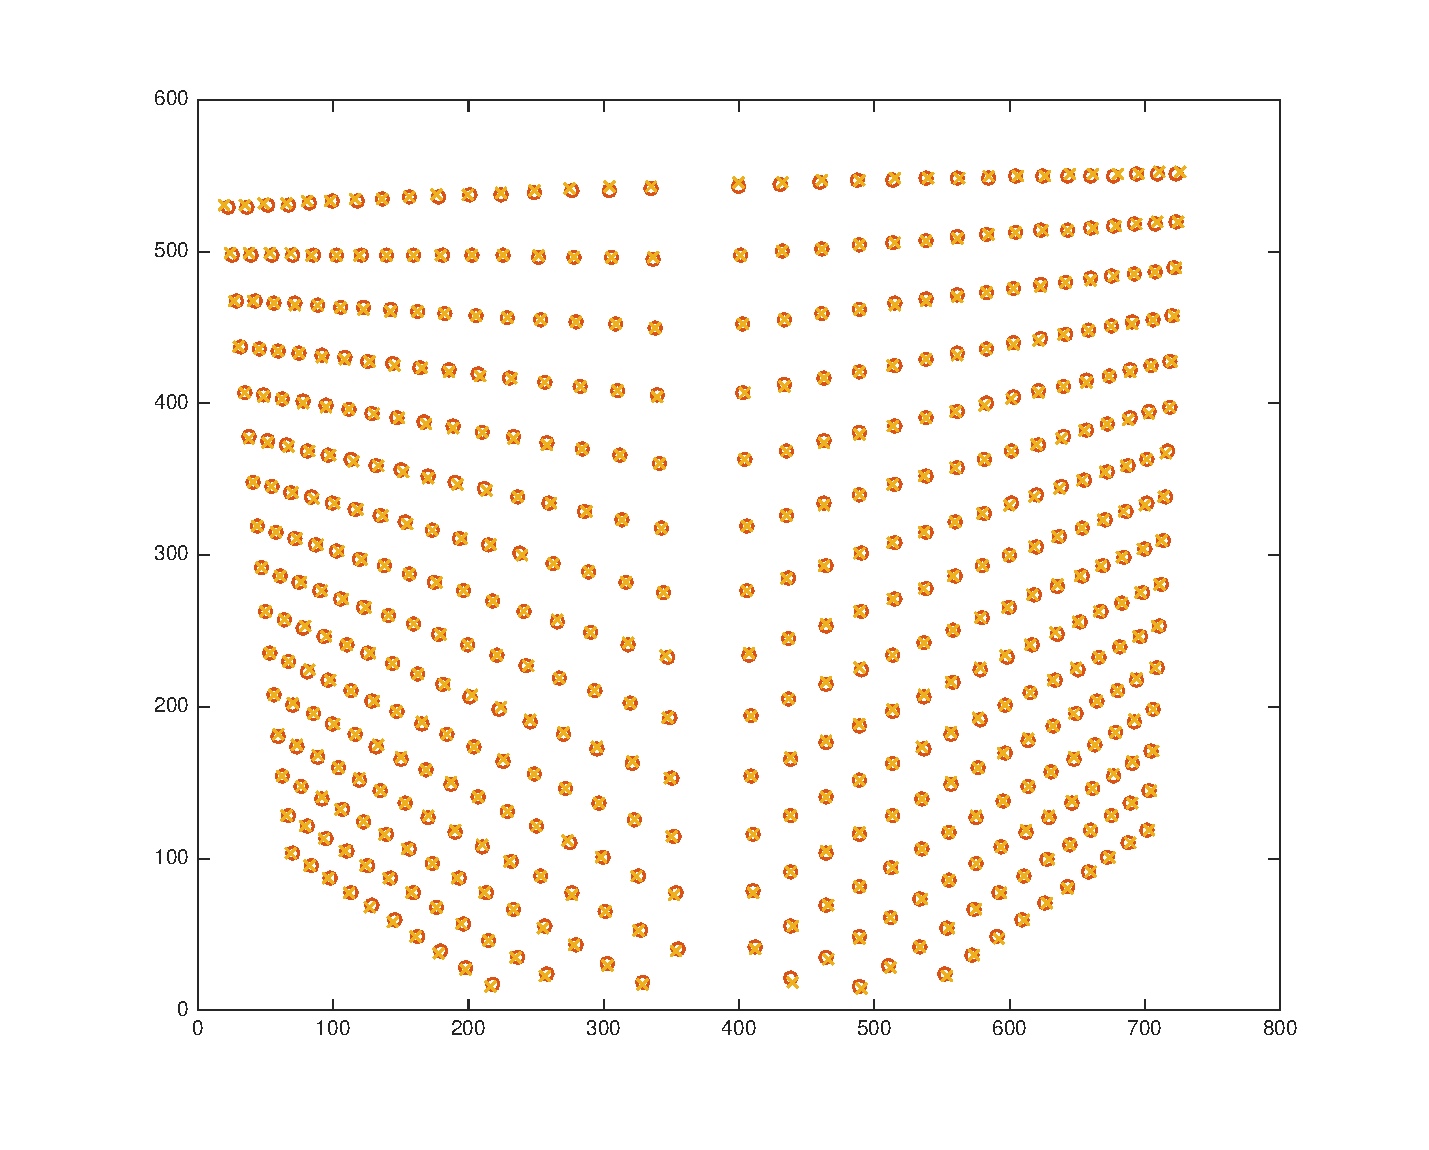
\includegraphics[width=\textwidth]{result.eps}
\caption{The original input points (circles) and the reprojected ones (crosses).}
\end{figure}

\end{document}